\section{Aufbau}
\label{sec:Aufbau}

Für den Versuch wird ein koaxialer Germaniumdektektor verwendet. Der Querschnitt des Detektors ist in Abbildung \ref{fig:aufbau} zu sehen.

\begin{figure}[H]
    \centering
    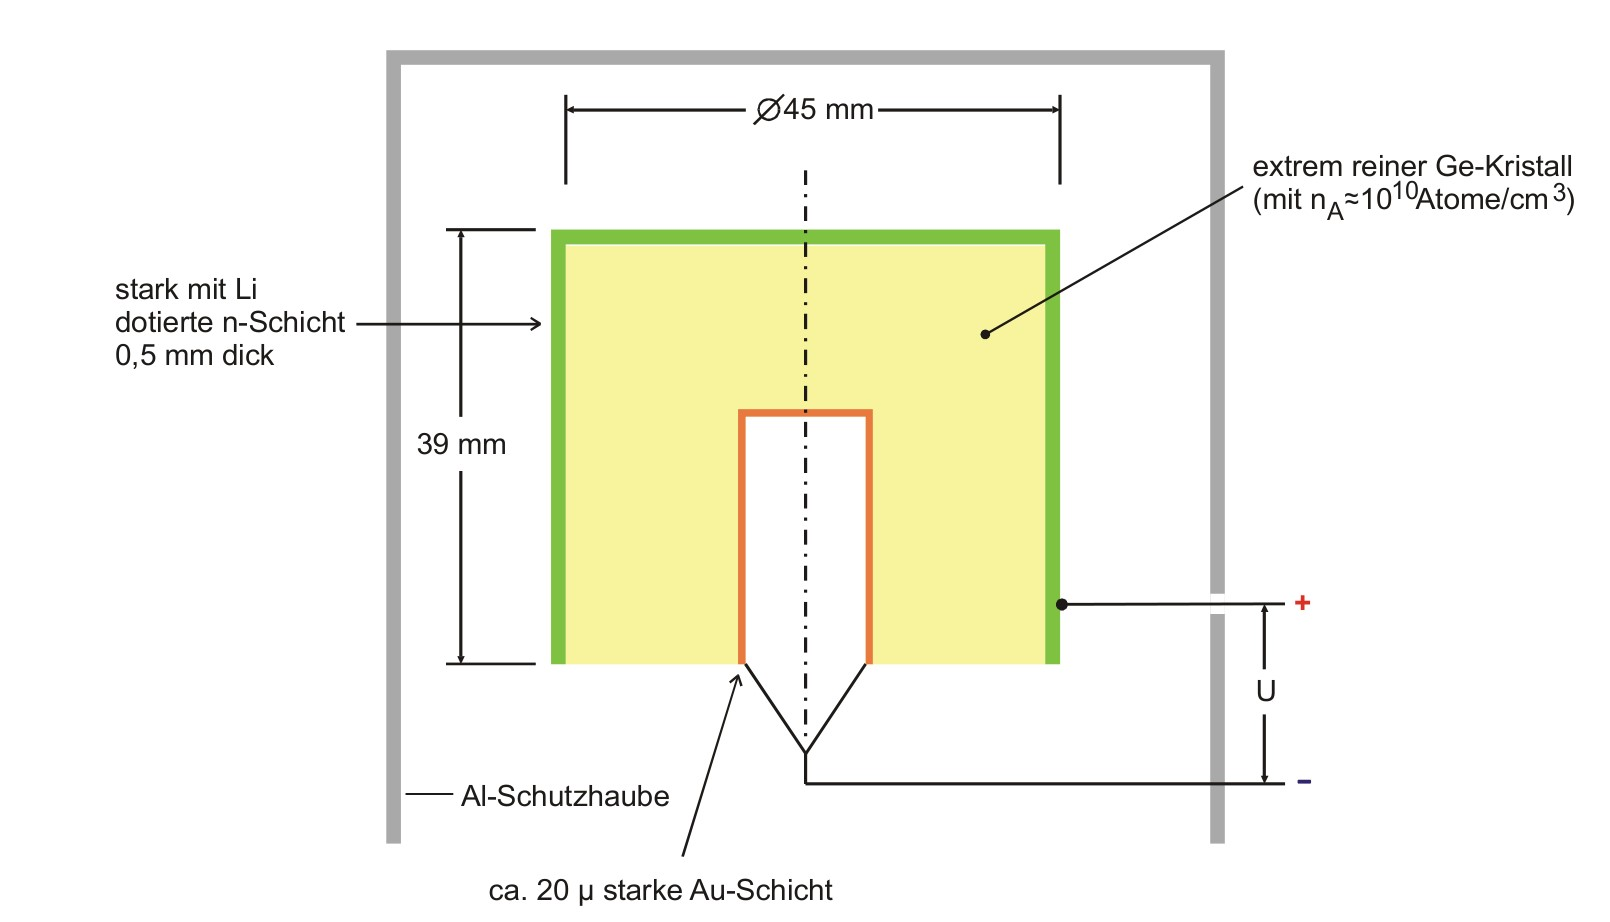
\includegraphics[width=0.8\textwidth]{content/grafik/aufbau.jpg}
    \caption{Der Querschnitt eines koaxialen Germaniumdektektors. \cite{germanium}}
    \label{fig:aufbau}
\end{figure}

Der Detektor ist zylinderförmig und hat einen Durchmesser $d$ = \qty{45}{\milli\meter} und eine Länge $l$ von \qty{39}{\milli\meter}.

